%%%%%%%%%%%%%%%%%%%%%%%%%%%%%%%%
%%% 演習4
%%%%%%%%%%%%%%%%%%%%%%%%%%%%%%%%

\exercises{4}{拡大縮小するウィンドウ}{
	ウィンドウサイズを2倍にしたら,ウィンドウ中の図形が2倍に拡大されて見えるような
	リサイズコールバック関数を作成せよ.
	ただし,ウィンドウの縦横比が変化しても,描画される図形の縦横比が変わらないようにせよ.
	例えばウィンドウサイズが$300 \times 200$画素のときは,
	WCSの$(-1.5, -1.0) \sim (1.5, 1.0)$の範囲が描画され,ウィンドウサイズが
	$200 \times 400$画素のときは,
	WCSの$(-1.0, -2.0) \sim (1.0, 2.0)$の範囲が描画されるような変換を考えればよい.
}

\vspace{\baselineskip}

% 文章

作成したリサイズコールバック関数を\Lstref{lst:ex04}に示す.
この関数はワールド座標系の矩形領域(\texttt{WCS\_L},\texttt{WCS\_B})$\sim$(\texttt{WCS\_R},\texttt{WCS\_T})
ウィンドウにギリギリ収まるように表示する.
ワールド座標系の表示する領域を設定できるため,汎用性が高く他のプログラムに応用しやすくなっている.
縦に余裕があるときの描画例と横に余裕があるときの描画例を\Figref{fig:ex04}に示す.
灰色の線は表示したい領域を示している.
ウィンドウにギリギリ収まるように描画できていることがわかる.

\lstinputlisting[
	caption = リサイズコールバック関数(\texttt{resize}),
	label = lst:ex04,
	linerange = {30-33, 35-37, 39-58}
]{
	../../Exercises/ex04.c
}

\begin{figure}[htbp]
	\centering
	\begin{minipage}[b]{0.4\textwidth}
		\centering
		
\includegraphics[scale=0.3]{../../Exercises/data/ex04-1.png}\\
		{\small (a) \; 縦に余裕があるとき}
	\end{minipage}
	\begin{minipage}[b]{0.5\textwidth}
		\centering
		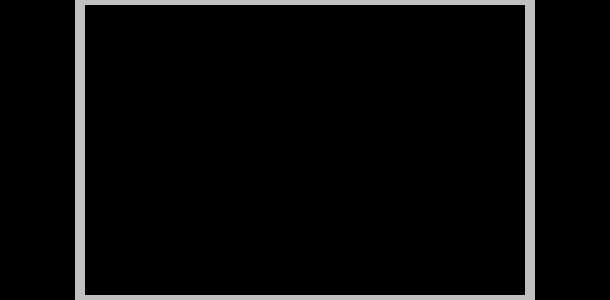
\includegraphics[scale=0.3]{../../Exercises/data/ex04-2.png}\\
		{\small (b) \; 横に余裕があるとき}
	\end{minipage}
	\label{fig:ex04}
	\caption{ウィンドウサイズ別の描画例}
\end{figure}
